\chapter{字符串算法}

本章讨论高效的字符串处理算法。许多字符串问题很容易在 $O(n^2)$ 时间内解决，而真正的挑战是找到时间复杂度为 $O(n)$ 或 $O(n \log n)$ 的算法。

\index{pattern matching}

例如，字符串处理中的一个基本问题是\key{模式匹配}：给定一个长度为 $n$ 的字符串和一个长度为 $m$ 的模式串，找出模式串在该字符串中的所有出现位置。例如，模式串 \texttt{ABC} 在字符串 \texttt{ABABCBABC} 中出现两次。

模式匹配很容易用暴力算法在 $O(nm)$ 时间内解决：逐一检查模式串可能出现的所有位置。不过，本章将介绍只需 $O(n+m)$ 时间的更高效算法。

\index{string}

\section{字符串术语}

\index{alphabet}

本章假设字符串采用从 0 开始的下标。因此，长度为 $n$ 的字符串 \texttt{s} 由字符 $\texttt{s}[0],\texttt{s}[1],\ldots,\texttt{s}[n-1]$ 组成。字符串中可能出现的字符集合称为\key{字符集}。例如，字符集 $\{\texttt{A},\texttt{B},\ldots,\texttt{Z}\}$ 由英语大写字母组成。

\index{substring}

\key{子串}是字符串中一段连续的字符序列。记号 $\texttt{s}[a \ldots b]$ 表示 \texttt{s} 中从位置 $a$ 开始、到位置 $b$ 结束的子串。长度为 $n$ 的字符串共有 $n(n+1)/2$ 个子串。例如，\texttt{ABCD} 的子串为
\texttt{A}, \texttt{B}, \texttt{C}, \texttt{D},
\texttt{AB}, \texttt{BC}, \texttt{CD},
\texttt{ABC}, \texttt{BCD} and \texttt{ABCD}.

\index{subsequence}

\key{子序列}是从字符串中按原有顺序取出的一列字符，这些字符不必连续。长度为 $n$ 的字符串共有 $2^n-1$ 个非空子序列。例如，\texttt{ABCD} 的子序列为
\texttt{A}, \texttt{B}, \texttt{C}, \texttt{D},
\texttt{AB}, \texttt{AC}, \texttt{AD},
\texttt{BC}, \texttt{BD}, \texttt{CD},
\texttt{ABC}, \texttt{ABD}, \texttt{ACD},
\texttt{BCD} and \texttt{ABCD}.

\index{prefix}
\index{suffix}

\key{前缀}是从字符串开头开始的子串，\key{后缀}是到字符串末尾结束的子串。例如，\texttt{ABCD} 的前缀为
\texttt{A}, \texttt{AB}, \texttt{ABC} and \texttt{ABCD},
而后缀为
\texttt{D}, \texttt{CD}, \texttt{BCD} and \texttt{ABCD}.

\index{rotation}

把字符串开头的字符依次移到末尾（或反过来），即可生成字符串的\key{循环移位}。例如，\texttt{ABCD} 的所有循环移位为
\texttt{ABCD}, \texttt{BCDA}, \texttt{CDAB} and \texttt{DABC}.

\index{period}

字符串的\key{周期}是一个前缀，重复这个前缀即可构造出原字符串；最后一次重复可以不完整，只包含该周期的一个前缀。例如，\texttt{ABCABCA} 的最短周期是 \texttt{ABC}。

\index{border}

若一个字符串同时是某字符串的前缀和后缀，就称它为该字符串的\key{border（边界）}。例如，\texttt{ABACABA} 的 border 为 \texttt{A}、\texttt{ABA} 和 \texttt{ABACABA}。

\index{lexicographical order}

字符串采用\key{字典序}（与字母表顺序对应）进行比较。若 $x \neq y$ 且 $x$ 是 $y$ 的前缀，或者存在位置 $k$，使得对所有 $i<k$ 都有 $x[i]=y[i]$ 且 $x[k]<y[k]$，则 $x<y$。

\section{Trie 结构}

\index{trie}

\key{Trie（字典树）}是一棵维护字符串集合的有根树。集合中的每个字符串都存储为一条从根节点开始的字符链。若两个字符串拥有公共前缀，它们在树中也会共享一段链。

例如，考虑下面的 Trie：

\begin{center}
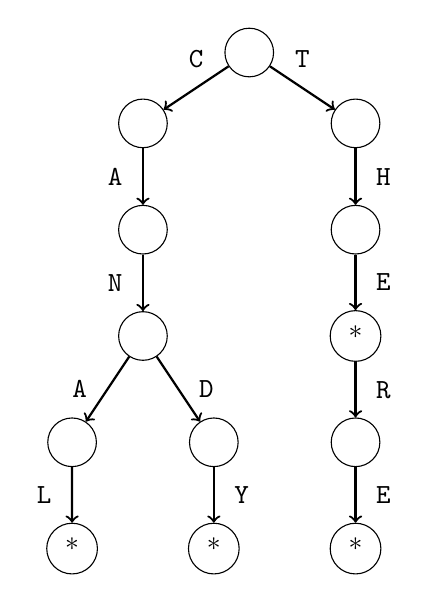
\begin{tikzpicture}[scale=0.9]
\node[draw, circle] (1) at (0,20) {$\phantom{1}$};
\node[draw, circle] (2) at (-1.5,19) {$\phantom{1}$};
\node[draw, circle] (3) at (1.5,19) {$\phantom{1}$};
\node[draw, circle] (4) at (-1.5,17.5) {$\phantom{1}$};
\node[draw, circle] (5) at (-1.5,16) {$\phantom{1}$};
\node[draw, circle] (6) at (-2.5,14.5) {$\phantom{1}$};
\node[draw, circle] (7) at (-0.5,14.5) {$\phantom{1}$};
\node[draw, circle] (8) at (-2.5,13) {*};
\node[draw, circle] (9) at (-0.5,13) {*};
\node[draw, circle] (10) at (1.5,17.5) {$\phantom{1}$};
\node[draw, circle] (11) at (1.5,16) {*};
\node[draw, circle] (12) at (1.5,14.5) {$\phantom{1}$};
\node[draw, circle] (13) at (1.5,13) {*};

\path[draw,thick,->] (1) -- node[font=\small,label=\texttt{C}] {} (2);
\path[draw,thick,->] (1) -- node[font=\small,label=\texttt{T}] {} (3);
\path[draw,thick,->] (2) -- node[font=\small,label=left:\texttt{A}] {} (4);
\path[draw,thick,->] (4) -- node[font=\small,label=left:\texttt{N}] {} (5);
\path[draw,thick,->] (5) -- node[font=\small,label=left:\texttt{A}] {} (6);
\path[draw,thick,->] (5) -- node[font=\small,label=right:\texttt{D}] {} (7);
\path[draw,thick,->] (6) -- node[font=\small,label=left:\texttt{L}] {}(8);
\path[draw,thick,->] (7) -- node[font=\small,label=right:\texttt{Y}] {} (9);
\path[draw,thick,->] (3) -- node[font=\small,label=right:\texttt{H}] {} (10);
\path[draw,thick,->] (10) -- node[font=\small,label=right:\texttt{E}] {} (11);
\path[draw,thick,->] (11) -- node[font=\small,label=right:\texttt{R}] {} (12);
\path[draw,thick,->] (12) -- node[font=\small,label=right:\texttt{E}] {} (13);
\end{tikzpicture}
\end{center}

该 Trie 对应集合 $\{\texttt{CANAL},\texttt{CANDY},\texttt{THE},\texttt{THERE}\}$。节点中的字符 * 表示集合中有一个字符串在该节点结束。这个标记是必需的，因为一个字符串可能是另一个字符串的前缀。例如，在上面的 Trie 中，\texttt{THE} 是 \texttt{THERE} 的前缀。

要判断 Trie 中是否包含一个长度为 $n$ 的字符串，只需沿着从根节点开始的链行进，时间复杂度为 $O(n)$。向 Trie 中加入一个长度为 $n$ 的字符串同样只需 $O(n)$ 时间：先沿已有链行进，再按需添加新节点。

利用 Trie，可以找出给定字符串中属于该集合的最长前缀。此外，若在每个节点中存储附加信息，还能计算集合中以给定字符串为前缀的字符串数量。

Trie 可以存储在数组中：
\begin{lstlisting}
int trie[N][A];
\end{lstlisting}
其中 $N$ 是节点数上限（即集合中所有字符串的总长度上限），$A$ 是字符集大小。Trie 的节点依次编号为 $0,1,2,\ldots$，根节点编号为 0；$\texttt{trie}[s][c]$ 表示从节点 $s$ 沿字符 $c$ 转移后到达的下一个节点。

\section{字符串哈希}

\index{hashing}
\index{string hashing}

\key{字符串哈希}是一种高效判断两个字符串是否相等的技术\footnote{该技术因 Karp--Rabin 模式匹配算法 \cite{kar87} 而得到推广。}。其思想是比较字符串的哈希值，而不是逐个比较字符。

\subsubsection*{计算哈希值}

\index{hash value}
\index{polynomial hashing}

字符串的\key{哈希值}是根据其中的字符计算得到的一个数。如果两个字符串相同，它们的哈希值也必然相同，因此可以借助哈希值比较字符串。

实现字符串哈希的常见方法是\key{多项式哈希}。长度为 $n$ 的字符串 \texttt{s} 的哈希值为
\[(\texttt{s}[0] A^{n-1} + \texttt{s}[1] A^{n-2} + \cdots + \texttt{s}[n-1] A^0) \bmod B  ,\]
其中 $s[0],s[1],\ldots,s[n-1]$ 解释为 \texttt{s} 中各字符的编码，$A$ 和 $B$ 是预先选定的常数。

例如，\texttt{ALLEY} 中各字符的编码为：
\begin{center}
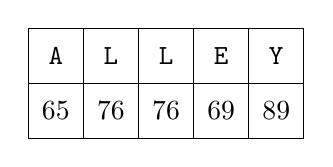
\begin{tikzpicture}[scale=0.7]
\draw (0,0) grid (5,2);

\node at (0.5, 1.5) {\texttt{A}};
\node at (1.5, 1.5) {\texttt{L}};
\node at (2.5, 1.5) {\texttt{L}};
\node at (3.5, 1.5) {\texttt{E}};
\node at (4.5, 1.5) {\texttt{Y}};

\node at (0.5, 0.5) {65};
\node at (1.5, 0.5) {76};
\node at (2.5, 0.5) {76};
\node at (3.5, 0.5) {69};
\node at (4.5, 0.5) {89};

\end{tikzpicture}
\end{center}

因此，当 $A=3$、$B=97$ 时，\texttt{ALLEY} 的哈希值为
\[(65 \cdot 3^4 + 76 \cdot 3^3 + 76 \cdot 3^2 + 69 \cdot 3^1 + 89 \cdot 3^0) \bmod 97 = 52.\]

\subsubsection*{预处理}

采用多项式哈希后，只需先进行 $O(n)$ 的预处理，就能在 $O(1)$ 时间内计算字符串 \texttt{s} 的任意子串哈希值。具体做法是构造数组 \texttt{h}，使 $\texttt{h}[k]$ 存储前缀 $\texttt{s}[0 \ldots k]$ 的哈希值。数组元素可按如下递推式计算：
\[
\begin{array}{lcl}
\texttt{h}[0] & = & \texttt{s}[0] \\
\texttt{h}[k] & = & (\texttt{h}[k-1] A + \texttt{s}[k]) \bmod B \\
\end{array}
\]
此外，构造数组 $\texttt{p}$，其中 $\texttt{p}[k]=A^k \bmod B$：
\[
\begin{array}{lcl}
\texttt{p}[0] & = & 1 \\
\texttt{p}[k] & = & (\texttt{p}[k-1] A) \bmod B. \\
\end{array}
\]
构造这两个数组需要 $O(n)$ 时间。随后，任意子串 $\texttt{s}[a \ldots b]$ 的哈希值都可在 $O(1)$ 时间内用下式计算：
\[(\texttt{h}[b]-\texttt{h}[a-1] \texttt{p}[b-a+1]) \bmod B\]
这里假设 $a>0$。若 $a=0$，哈希值就是 $\texttt{h}[b]$。

\subsubsection*{使用哈希值}

借助哈希值，可以高效比较字符串。其思想是不再逐个比较字符，而是比较两个字符串的哈希值。若哈希值相等，字符串\emph{很可能}相等；若哈希值不同，字符串则\emph{一定}不同。

哈希常常能让暴力算法变得高效。以模式匹配为例：给定字符串 $s$ 和模式串 $p$，找出 $p$ 在 $s$ 中出现的位置。暴力算法枚举 $p$ 可能出现的所有位置，再逐字符比较，时间复杂度为 $O(n^2)$。

由于该算法实际比较的是字符串的子串，可以用哈希提升效率。采用哈希后，每次只比较子串的哈希值，因而只需 $O(1)$ 时间。最终算法的时间复杂度为 $O(n)$，这也是该问题可能达到的最优时间复杂度。

将哈希与\emph{二分查找}结合，还可以在对数时间内确定两个字符串的字典序。先通过二分查找计算两字符串公共前缀的长度，再比较公共前缀之后的第一个字符，即可确定顺序。

\subsubsection*{冲突与参数}

\index{collision}

比较哈希值时，一个明显风险是发生\key{哈希冲突}：两个内容不同的字符串却具有相同哈希值。此时，依赖哈希值的算法会误以为字符串相等，从而可能给出错误结果。

由于不同字符串的数量大于不同哈希值的数量，冲突始终可能发生。不过，只要谨慎选择常数 $A$ 和 $B$，冲突概率就会很小。常见做法是在 $10^9$ 附近随机选取常数，例如：
\[
\begin{array}{lcl}
A & = & 911382323 \\
B & = & 972663749 \\
\end{array}
\]

采用这样的常数计算哈希值时，可以使用 \texttt{long long} 类型，因为乘积 $AB$ 和 $BB$ 都能容纳在 \texttt{long long} 中。但大约 $10^9$ 种不同哈希值真的足够吗？

考虑使用哈希的三种情形：

\textit{情形 1：}比较字符串 $x$ 与 $y$。假设所有哈希值等概率出现，发生冲突的概率为 $1/B$。

\textit{情形 2：}把字符串 $x$ 分别与字符串 $y_1,y_2,\ldots,y_n$ 比较。至少发生一次冲突的概率为

\[1-(1-\frac{1}{B})^n.\]

\textit{情形 3：}比较字符串 $x_1,x_2,\ldots,x_n$ 的所有两两组合。至少发生一次冲突的概率为
\[ 1 - \frac{B \cdot (B-1) \cdot (B-2) \cdots (B-n+1)}{B^n}.\]

下表给出 $n=10^6$ 且 $B$ 取不同值时的冲突概率：

\begin{center}
\begin{tabular}{rrrr}
常数 $B$ & 情形 1 & 情形 2 & 情形 3 \\
\hline
$10^3$ & $0.001000$ & $1.000000$ & $1.000000$ \\
$10^6$ & $0.000001$ & $0.632121$ & $1.000000$ \\
$10^9$ & $0.000000$ & $0.001000$ & $1.000000$ \\
$10^{12}$ & $0.000000$ & $0.000000$ & $0.393469$ \\
$10^{15}$ & $0.000000$ & $0.000000$ & $0.000500$ \\
$10^{18}$ & $0.000000$ & $0.000000$ & $0.000001$ \\
\end{tabular}
\end{center}

表中可以看出，在情形 1 中，当 $B \approx 10^9$ 时冲突概率可以忽略不计。情形 2 中可能发生冲突，但概率仍然很小。然而情形 3 完全不同：当 $B \approx 10^9$ 时，几乎必然发生冲突。

\index{birthday paradox}

情形 3 中的现象称为\key{生日悖论}：一个房间里有 $n$ 个人，即使 $n$ 不大，\emph{某两个人}生日相同的概率也会很高。对应到哈希中，当所有哈希值两两比较时，存在两个相同哈希值的概率很大。

使用不同参数计算\emph{多组}哈希值，可以降低冲突概率。所有哈希值同时发生冲突的可能性很低。例如，两组参数 $B \approx 10^9$ 的哈希值，大致相当于一组参数 $B \approx 10^{18}$ 的哈希值，冲突概率因而非常小。

有些人使用常数 $B=2^{32}$ 或 $B=2^{64}$，这样做很方便，因为 32 位和 64 位整数运算会自然地分别对 $2^{32}$ 和 $2^{64}$ 取模。然而，这\emph{不是}一个好选择：当常数形如 $2^x$ 时，可以构造出必然产生冲突的输入 \cite{pac13}。

\section{Z 算法}

\index{Z-algorithm}
\index{Z-array}

长度为 $n$ 的字符串 \texttt{s} 的\key{Z 数组} \texttt{z}，对每个 $k=0,1,\ldots,n-1$，记录从位置 $k$ 开始且同时是 \texttt{s} 前缀的最长子串长度。因此，$\texttt{z}[k]=p$ 表示 $\texttt{s}[0 \ldots p-1]$ 与 $\texttt{s}[k \ldots k+p-1]$ 相等。利用 Z 数组可以高效解决许多字符串处理问题。

例如，\texttt{ACBACDACBACBACDA} 的 Z 数组如下：

\begin{center}
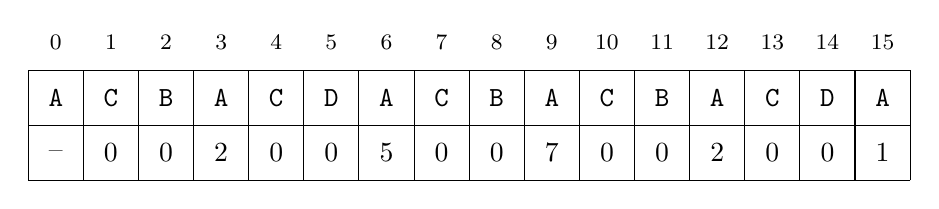
\begin{tikzpicture}[scale=0.7]
\draw (0,0) grid (16,2);

\node at (0.5, 1.5) {\texttt{A}};
\node at (1.5, 1.5) {\texttt{C}};
\node at (2.5, 1.5) {\texttt{B}};
\node at (3.5, 1.5) {\texttt{A}};
\node at (4.5, 1.5) {\texttt{C}};
\node at (5.5, 1.5) {\texttt{D}};
\node at (6.5, 1.5) {\texttt{A}};
\node at (7.5, 1.5) {\texttt{C}};
\node at (8.5, 1.5) {\texttt{B}};
\node at (9.5, 1.5) {\texttt{A}};
\node at (10.5, 1.5) {\texttt{C}};
\node at (11.5, 1.5) {\texttt{B}};
\node at (12.5, 1.5) {\texttt{A}};
\node at (13.5, 1.5) {\texttt{C}};
\node at (14.5, 1.5) {\texttt{D}};
\node at (15.5, 1.5) {\texttt{A}};

\node at (0.5, 0.5) {--};
\node at (1.5, 0.5) {0};
\node at (2.5, 0.5) {0};
\node at (3.5, 0.5) {2};
\node at (4.5, 0.5) {0};
\node at (5.5, 0.5) {0};
\node at (6.5, 0.5) {5};
\node at (7.5, 0.5) {0};
\node at (8.5, 0.5) {0};
\node at (9.5, 0.5) {7};
\node at (10.5, 0.5) {0};
\node at (11.5, 0.5) {0};
\node at (12.5, 0.5) {2};
\node at (13.5, 0.5) {0};
\node at (14.5, 0.5) {0};
\node at (15.5, 0.5) {1};

\footnotesize
\node at (0.5, 2.5) {0};
\node at (1.5, 2.5) {1};
\node at (2.5, 2.5) {2};
\node at (3.5, 2.5) {3};
\node at (4.5, 2.5) {4};
\node at (5.5, 2.5) {5};
\node at (6.5, 2.5) {6};
\node at (7.5, 2.5) {7};
\node at (8.5, 2.5) {8};
\node at (9.5, 2.5) {9};
\node at (10.5, 2.5) {10};
\node at (11.5, 2.5) {11};
\node at (12.5, 2.5) {12};
\node at (13.5, 2.5) {13};
\node at (14.5, 2.5) {14};
\node at (15.5, 2.5) {15};

\end{tikzpicture}
\end{center}

例如，此处 $\texttt{z}[6]=5$，因为长度为 5 的子串 \texttt{ACBAC} 是 \texttt{s} 的前缀，而长度为 6 的子串 \texttt{ACBACB} 不是其前缀。

\subsubsection*{算法说明}

下面介绍\key{Z 算法}\footnote{文献 \cite{gus97} 把 Z 算法描述为已知最简单的线性时间模式匹配方法，并将最初的思想归于文献 \cite{mai84}。}，它能在 $O(n)$ 时间内高效构造 Z 数组。算法从左到右计算 Z 数组，既利用数组中已经存储的信息，也在必要时逐字符比较子串。

为了高效计算 Z 数组，算法维护区间 $[x,y]$，使得 $\texttt{s}[x \ldots y]$ 是 \texttt{s} 的前缀，并且 $y$ 尽可能大。由于已知 $\texttt{s}[0 \ldots y-x]$ 与 $\texttt{s}[x \ldots y]$ 相等，计算位置 $x+1,x+2,\ldots,y$ 的 Z 值时便可以利用这一信息。

在每个位置 $k$，先检查 $\texttt{z}[k-x]$。若 $k+\texttt{z}[k-x]<y$，就能确定 $\texttt{z}[k]=\texttt{z}[k-x]$。若 $k+\texttt{z}[k-x] \ge y$，则已知 $\texttt{s}[0 \ldots y-k]$ 与 $\texttt{s}[k \ldots y]$ 相等；为了确定 $\texttt{z}[k]$，还需继续逐字符比较子串。算法仍然只需 $O(n)$ 时间，因为比较从位置 $y-k+1$ 和 $y+1$ 开始。

例如，下面构造这个 Z 数组：

\begin{center}
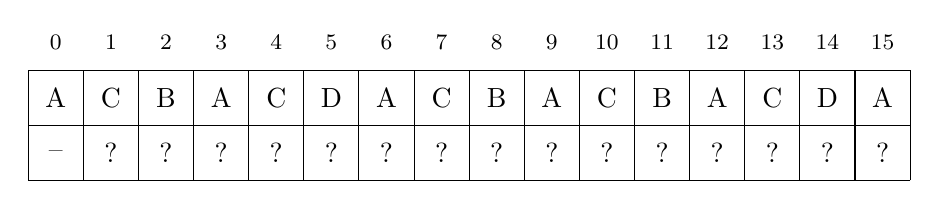
\begin{tikzpicture}[scale=0.7]
\draw (0,0) grid (16,2);

\node at (0.5, 1.5) {A};
\node at (1.5, 1.5) {C};
\node at (2.5, 1.5) {B};
\node at (3.5, 1.5) {A};
\node at (4.5, 1.5) {C};
\node at (5.5, 1.5) {D};
\node at (6.5, 1.5) {A};
\node at (7.5, 1.5) {C};
\node at (8.5, 1.5) {B};
\node at (9.5, 1.5) {A};
\node at (10.5, 1.5) {C};
\node at (11.5, 1.5) {B};
\node at (12.5, 1.5) {A};
\node at (13.5, 1.5) {C};
\node at (14.5, 1.5) {D};
\node at (15.5, 1.5) {A};

\node at (0.5, 0.5) {--};
\node at (1.5, 0.5) {?};
\node at (2.5, 0.5) {?};
\node at (3.5, 0.5) {?};
\node at (4.5, 0.5) {?};
\node at (5.5, 0.5) {?};
\node at (6.5, 0.5) {?};
\node at (7.5, 0.5) {?};
\node at (8.5, 0.5) {?};
\node at (9.5, 0.5) {?};
\node at (10.5, 0.5) {?};
\node at (11.5, 0.5) {?};
\node at (12.5, 0.5) {?};
\node at (13.5, 0.5) {?};
\node at (14.5, 0.5) {?};
\node at (15.5, 0.5) {?};

\footnotesize
\node at (0.5, 2.5) {0};
\node at (1.5, 2.5) {1};
\node at (2.5, 2.5) {2};
\node at (3.5, 2.5) {3};
\node at (4.5, 2.5) {4};
\node at (5.5, 2.5) {5};
\node at (6.5, 2.5) {6};
\node at (7.5, 2.5) {7};
\node at (8.5, 2.5) {8};
\node at (9.5, 2.5) {9};
\node at (10.5, 2.5) {10};
\node at (11.5, 2.5) {11};
\node at (12.5, 2.5) {12};
\node at (13.5, 2.5) {13};
\node at (14.5, 2.5) {14};
\node at (15.5, 2.5) {15};

\end{tikzpicture}
\end{center}

计算出 $\texttt{z}[6]=5$ 后，当前的 $[x,y]$ 区间为 $[6,10]$：

\begin{center}
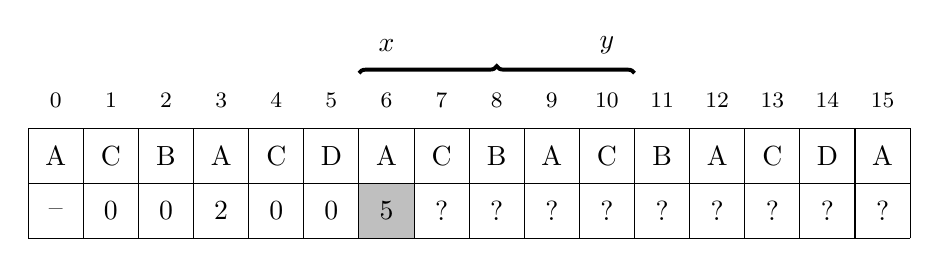
\begin{tikzpicture}[scale=0.7]
\fill[color=lightgray] (6,0) rectangle (7,1);
\draw (0,0) grid (16,2);

\node at (0.5, 1.5) {A};
\node at (1.5, 1.5) {C};
\node at (2.5, 1.5) {B};
\node at (3.5, 1.5) {A};
\node at (4.5, 1.5) {C};
\node at (5.5, 1.5) {D};
\node at (6.5, 1.5) {A};
\node at (7.5, 1.5) {C};
\node at (8.5, 1.5) {B};
\node at (9.5, 1.5) {A};
\node at (10.5, 1.5) {C};
\node at (11.5, 1.5) {B};
\node at (12.5, 1.5) {A};
\node at (13.5, 1.5) {C};
\node at (14.5, 1.5) {D};
\node at (15.5, 1.5) {A};

\node at (0.5, 0.5) {--};
\node at (1.5, 0.5) {0};
\node at (2.5, 0.5) {0};
\node at (3.5, 0.5) {2};
\node at (4.5, 0.5) {0};
\node at (5.5, 0.5) {0};
\node at (6.5, 0.5) {5};
\node at (7.5, 0.5) {?};
\node at (8.5, 0.5) {?};
\node at (9.5, 0.5) {?};
\node at (10.5, 0.5) {?};
\node at (11.5, 0.5) {?};
\node at (12.5, 0.5) {?};
\node at (13.5, 0.5) {?};
\node at (14.5, 0.5) {?};
\node at (15.5, 0.5) {?};

\draw [decoration={brace}, decorate, line width=0.5mm] (6,3.00) -- (11,3.00);

\node at (6.5,3.50) {$x$};
\node at (10.5,3.50) {$y$};


\footnotesize
\node at (0.5, 2.5) {0};
\node at (1.5, 2.5) {1};
\node at (2.5, 2.5) {2};
\node at (3.5, 2.5) {3};
\node at (4.5, 2.5) {4};
\node at (5.5, 2.5) {5};
\node at (6.5, 2.5) {6};
\node at (7.5, 2.5) {7};
\node at (8.5, 2.5) {8};
\node at (9.5, 2.5) {9};
\node at (10.5, 2.5) {10};
\node at (11.5, 2.5) {11};
\node at (12.5, 2.5) {12};
\node at (13.5, 2.5) {13};
\node at (14.5, 2.5) {14};
\node at (15.5, 2.5) {15};

\end{tikzpicture}
\end{center}

现在已知 $\texttt{s}[0 \ldots 4]$ 与 $\texttt{s}[6 \ldots 10]$ 相等，因此可以高效计算后续 Z 数组元素。首先，由于 $\texttt{z}[1] = \texttt{z}[2] = 0$，立即可知 $\texttt{z}[7] = \texttt{z}[8] = 0$：

\begin{center}
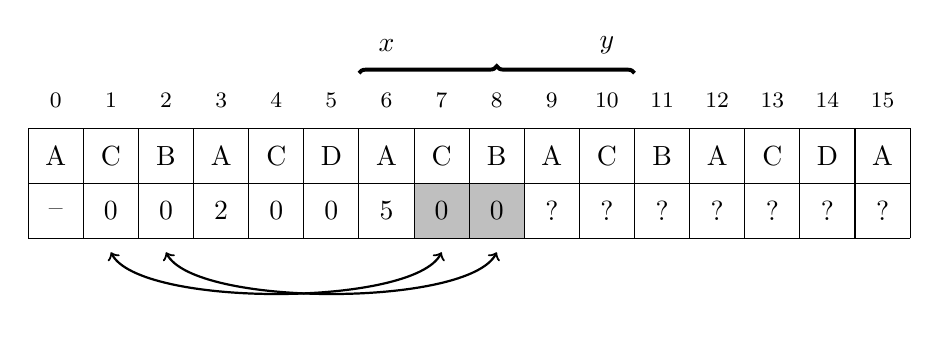
\begin{tikzpicture}[scale=0.7]
\fill[color=lightgray] (7,0) rectangle (9,1);
\draw (0,0) grid (16,2);

\node at (0.5, 1.5) {A};
\node at (1.5, 1.5) {C};
\node at (2.5, 1.5) {B};
\node at (3.5, 1.5) {A};
\node at (4.5, 1.5) {C};
\node at (5.5, 1.5) {D};
\node at (6.5, 1.5) {A};
\node at (7.5, 1.5) {C};
\node at (8.5, 1.5) {B};
\node at (9.5, 1.5) {A};
\node at (10.5, 1.5) {C};
\node at (11.5, 1.5) {B};
\node at (12.5, 1.5) {A};
\node at (13.5, 1.5) {C};
\node at (14.5, 1.5) {D};
\node at (15.5, 1.5) {A};

\node at (0.5, 0.5) {--};
\node at (1.5, 0.5) {0};
\node at (2.5, 0.5) {0};
\node at (3.5, 0.5) {2};
\node at (4.5, 0.5) {0};
\node at (5.5, 0.5) {0};
\node at (6.5, 0.5) {5};
\node at (7.5, 0.5) {0};
\node at (8.5, 0.5) {0};
\node at (9.5, 0.5) {?};
\node at (10.5, 0.5) {?};
\node at (11.5, 0.5) {?};
\node at (12.5, 0.5) {?};
\node at (13.5, 0.5) {?};
\node at (14.5, 0.5) {?};
\node at (15.5, 0.5) {?};


\draw [decoration={brace}, decorate, line width=0.5mm] (6,3.00) -- (11,3.00);

\node at (6.5,3.50) {$x$};
\node at (10.5,3.50) {$y$};


\footnotesize
\node at (0.5, 2.5) {0};
\node at (1.5, 2.5) {1};
\node at (2.5, 2.5) {2};
\node at (3.5, 2.5) {3};
\node at (4.5, 2.5) {4};
\node at (5.5, 2.5) {5};
\node at (6.5, 2.5) {6};
\node at (7.5, 2.5) {7};
\node at (8.5, 2.5) {8};
\node at (9.5, 2.5) {9};
\node at (10.5, 2.5) {10};
\node at (11.5, 2.5) {11};
\node at (12.5, 2.5) {12};
\node at (13.5, 2.5) {13};
\node at (14.5, 2.5) {14};
\node at (15.5, 2.5) {15};


\draw[thick,<->] (7.5,-0.25) .. controls (7,-1.25) and (2,-1.25) .. (1.5,-0.25);
\draw[thick,<->] (8.5,-0.25) .. controls (8,-1.25) and (3,-1.25) .. (2.5,-0.25);
\end{tikzpicture}
\end{center}

接着，由于 $\texttt{z}[3]=2$，可知 $\texttt{z}[9] \ge 2$：

\begin{center}
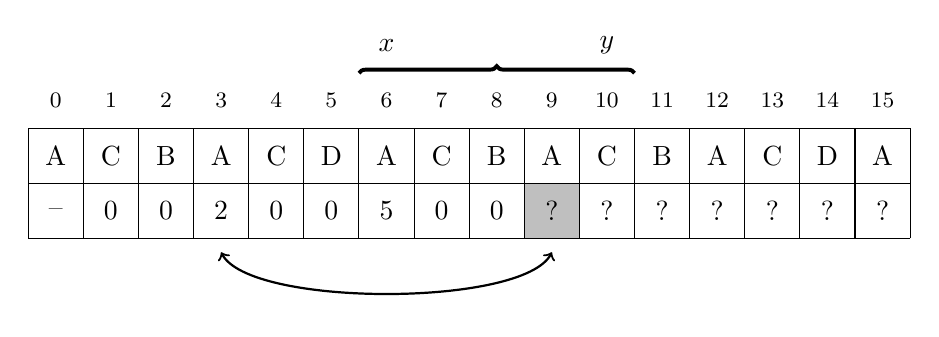
\begin{tikzpicture}[scale=0.7]
\fill[color=lightgray] (9,0) rectangle (10,1);
\draw (0,0) grid (16,2);

\node at (0.5, 1.5) {A};
\node at (1.5, 1.5) {C};
\node at (2.5, 1.5) {B};
\node at (3.5, 1.5) {A};
\node at (4.5, 1.5) {C};
\node at (5.5, 1.5) {D};
\node at (6.5, 1.5) {A};
\node at (7.5, 1.5) {C};
\node at (8.5, 1.5) {B};
\node at (9.5, 1.5) {A};
\node at (10.5, 1.5) {C};
\node at (11.5, 1.5) {B};
\node at (12.5, 1.5) {A};
\node at (13.5, 1.5) {C};
\node at (14.5, 1.5) {D};
\node at (15.5, 1.5) {A};

\node at (0.5, 0.5) {--};
\node at (1.5, 0.5) {0};
\node at (2.5, 0.5) {0};
\node at (3.5, 0.5) {2};
\node at (4.5, 0.5) {0};
\node at (5.5, 0.5) {0};
\node at (6.5, 0.5) {5};
\node at (7.5, 0.5) {0};
\node at (8.5, 0.5) {0};
\node at (9.5, 0.5) {?};
\node at (10.5, 0.5) {?};
\node at (11.5, 0.5) {?};
\node at (12.5, 0.5) {?};
\node at (13.5, 0.5) {?};
\node at (14.5, 0.5) {?};
\node at (15.5, 0.5) {?};

\draw [decoration={brace}, decorate, line width=0.5mm] (6,3.00) -- (11,3.00);

\node at (6.5,3.50) {$x$};
\node at (10.5,3.50) {$y$};


\footnotesize
\node at (0.5, 2.5) {0};
\node at (1.5, 2.5) {1};
\node at (2.5, 2.5) {2};
\node at (3.5, 2.5) {3};
\node at (4.5, 2.5) {4};
\node at (5.5, 2.5) {5};
\node at (6.5, 2.5) {6};
\node at (7.5, 2.5) {7};
\node at (8.5, 2.5) {8};
\node at (9.5, 2.5) {9};
\node at (10.5, 2.5) {10};
\node at (11.5, 2.5) {11};
\node at (12.5, 2.5) {12};
\node at (13.5, 2.5) {13};
\node at (14.5, 2.5) {14};
\node at (15.5, 2.5) {15};

\draw[thick,<->] (9.5,-0.25) .. controls (9,-1.25) and (4,-1.25) .. (3.5,-0.25);
\end{tikzpicture}
\end{center}

但是，我们没有位置 10 之后的字符串信息，因此需要逐字符比较子串：

\begin{center}
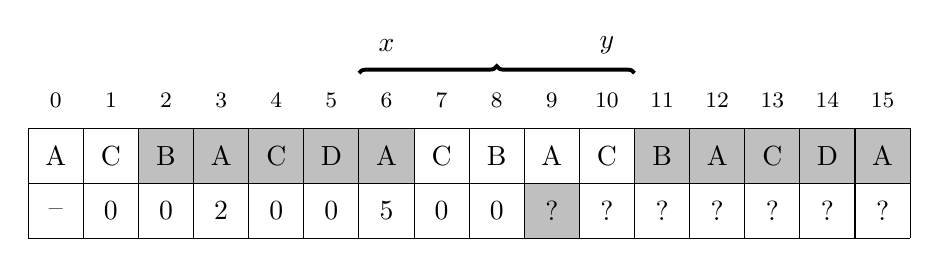
\begin{tikzpicture}[scale=0.7]
\fill[color=lightgray] (9,0) rectangle (10,1);
\fill[color=lightgray] (2,1) rectangle (7,2);
\fill[color=lightgray] (11,1) rectangle (16,2);


\draw (0,0) grid (16,2);

\node at (0.5, 1.5) {A};
\node at (1.5, 1.5) {C};
\node at (2.5, 1.5) {B};
\node at (3.5, 1.5) {A};
\node at (4.5, 1.5) {C};
\node at (5.5, 1.5) {D};
\node at (6.5, 1.5) {A};
\node at (7.5, 1.5) {C};
\node at (8.5, 1.5) {B};
\node at (9.5, 1.5) {A};
\node at (10.5, 1.5) {C};
\node at (11.5, 1.5) {B};
\node at (12.5, 1.5) {A};
\node at (13.5, 1.5) {C};
\node at (14.5, 1.5) {D};
\node at (15.5, 1.5) {A};

\node at (0.5, 0.5) {--};
\node at (1.5, 0.5) {0};
\node at (2.5, 0.5) {0};
\node at (3.5, 0.5) {2};
\node at (4.5, 0.5) {0};
\node at (5.5, 0.5) {0};
\node at (6.5, 0.5) {5};
\node at (7.5, 0.5) {0};
\node at (8.5, 0.5) {0};
\node at (9.5, 0.5) {?};
\node at (10.5, 0.5) {?};
\node at (11.5, 0.5) {?};
\node at (12.5, 0.5) {?};
\node at (13.5, 0.5) {?};
\node at (14.5, 0.5) {?};
\node at (15.5, 0.5) {?};

\draw [decoration={brace}, decorate, line width=0.5mm] (6,3.00) -- (11,3.00);

\node at (6.5,3.50) {$x$};
\node at (10.5,3.50) {$y$};


\footnotesize
\node at (0.5, 2.5) {0};
\node at (1.5, 2.5) {1};
\node at (2.5, 2.5) {2};
\node at (3.5, 2.5) {3};
\node at (4.5, 2.5) {4};
\node at (5.5, 2.5) {5};
\node at (6.5, 2.5) {6};
\node at (7.5, 2.5) {7};
\node at (8.5, 2.5) {8};
\node at (9.5, 2.5) {9};
\node at (10.5, 2.5) {10};
\node at (11.5, 2.5) {11};
\node at (12.5, 2.5) {12};
\node at (13.5, 2.5) {13};
\node at (14.5, 2.5) {14};
\node at (15.5, 2.5) {15};

%\draw[thick,<->] (11.5,-0.25) .. controls (11,-1.25) and (3,-1.25) .. (2.5,-0.25);
\end{tikzpicture}
\end{center}

结果得到 $\texttt{z}[9]=7$，于是新的 $[x,y]$ 区间为 $[9,15]$：

\begin{center}
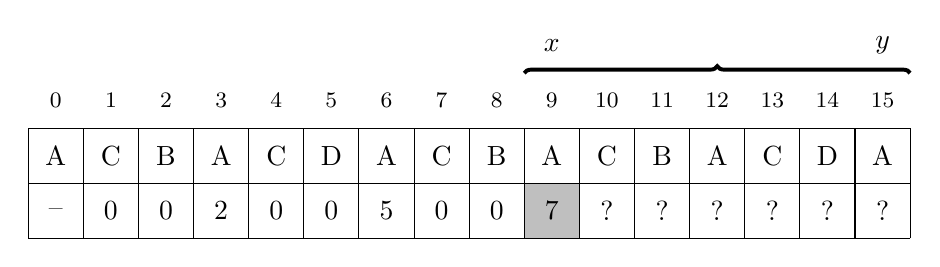
\begin{tikzpicture}[scale=0.7]
\fill[color=lightgray] (9,0) rectangle (10,1);
\draw (0,0) grid (16,2);

\node at (0.5, 1.5) {A};
\node at (1.5, 1.5) {C};
\node at (2.5, 1.5) {B};
\node at (3.5, 1.5) {A};
\node at (4.5, 1.5) {C};
\node at (5.5, 1.5) {D};
\node at (6.5, 1.5) {A};
\node at (7.5, 1.5) {C};
\node at (8.5, 1.5) {B};
\node at (9.5, 1.5) {A};
\node at (10.5, 1.5) {C};
\node at (11.5, 1.5) {B};
\node at (12.5, 1.5) {A};
\node at (13.5, 1.5) {C};
\node at (14.5, 1.5) {D};
\node at (15.5, 1.5) {A};

\node at (0.5, 0.5) {--};
\node at (1.5, 0.5) {0};
\node at (2.5, 0.5) {0};
\node at (3.5, 0.5) {2};
\node at (4.5, 0.5) {0};
\node at (5.5, 0.5) {0};
\node at (6.5, 0.5) {5};
\node at (7.5, 0.5) {0};
\node at (8.5, 0.5) {0};
\node at (9.5, 0.5) {7};
\node at (10.5, 0.5) {?};
\node at (11.5, 0.5) {?};
\node at (12.5, 0.5) {?};
\node at (13.5, 0.5) {?};
\node at (14.5, 0.5) {?};
\node at (15.5, 0.5) {?};

\draw [decoration={brace}, decorate, line width=0.5mm] (9,3.00) -- (16,3.00);

\node at (9.5,3.50) {$x$};
\node at (15.5,3.50) {$y$};


\footnotesize
\node at (0.5, 2.5) {0};
\node at (1.5, 2.5) {1};
\node at (2.5, 2.5) {2};
\node at (3.5, 2.5) {3};
\node at (4.5, 2.5) {4};
\node at (5.5, 2.5) {5};
\node at (6.5, 2.5) {6};
\node at (7.5, 2.5) {7};
\node at (8.5, 2.5) {8};
\node at (9.5, 2.5) {9};
\node at (10.5, 2.5) {10};
\node at (11.5, 2.5) {11};
\node at (12.5, 2.5) {12};
\node at (13.5, 2.5) {13};
\node at (14.5, 2.5) {14};
\node at (15.5, 2.5) {15};

% \draw[thick,<->] (9.5,-0.25) .. controls (9,-1.25) and (4,-1.25) .. (3.5,-0.25);
\end{tikzpicture}
\end{center}

此后，只需利用 Z 数组中已有的信息，就能确定其余所有元素：

\begin{center}
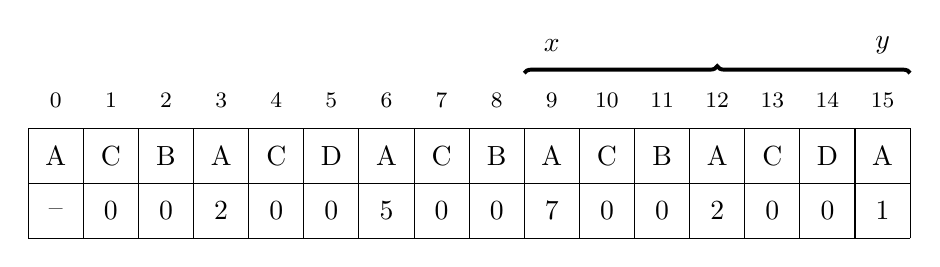
\begin{tikzpicture}[scale=0.7]
\draw (0,0) grid (16,2);

\node at (0.5, 1.5) {A};
\node at (1.5, 1.5) {C};
\node at (2.5, 1.5) {B};
\node at (3.5, 1.5) {A};
\node at (4.5, 1.5) {C};
\node at (5.5, 1.5) {D};
\node at (6.5, 1.5) {A};
\node at (7.5, 1.5) {C};
\node at (8.5, 1.5) {B};
\node at (9.5, 1.5) {A};
\node at (10.5, 1.5) {C};
\node at (11.5, 1.5) {B};
\node at (12.5, 1.5) {A};
\node at (13.5, 1.5) {C};
\node at (14.5, 1.5) {D};
\node at (15.5, 1.5) {A};

\node at (0.5, 0.5) {--};
\node at (1.5, 0.5) {0};
\node at (2.5, 0.5) {0};
\node at (3.5, 0.5) {2};
\node at (4.5, 0.5) {0};
\node at (5.5, 0.5) {0};
\node at (6.5, 0.5) {5};
\node at (7.5, 0.5) {0};
\node at (8.5, 0.5) {0};
\node at (9.5, 0.5) {7};
\node at (10.5, 0.5) {0};
\node at (11.5, 0.5) {0};
\node at (12.5, 0.5) {2};
\node at (13.5, 0.5) {0};
\node at (14.5, 0.5) {0};
\node at (15.5, 0.5) {1};

\draw [decoration={brace}, decorate, line width=0.5mm] (9,3.00) -- (16,3.00);

\node at (9.5,3.50) {$x$};
\node at (15.5,3.50) {$y$};


\footnotesize
\node at (0.5, 2.5) {0};
\node at (1.5, 2.5) {1};
\node at (2.5, 2.5) {2};
\node at (3.5, 2.5) {3};
\node at (4.5, 2.5) {4};
\node at (5.5, 2.5) {5};
\node at (6.5, 2.5) {6};
\node at (7.5, 2.5) {7};
\node at (8.5, 2.5) {8};
\node at (9.5, 2.5) {9};
\node at (10.5, 2.5) {10};
\node at (11.5, 2.5) {11};
\node at (12.5, 2.5) {12};
\node at (13.5, 2.5) {13};
\node at (14.5, 2.5) {14};
\node at (15.5, 2.5) {15};

\end{tikzpicture}
\end{center}

\subsubsection{使用 Z 数组}

选择字符串哈希还是 Z 算法，往往取决于个人偏好。与哈希不同，Z 算法总能给出确定结果，不存在冲突风险；另一方面，Z 算法更难实现，而且有些问题只能用哈希解决。

再次考虑模式匹配问题：找出模式串 $p$ 在字符串 $s$ 中的所有出现位置。前面已经用字符串哈希高效解决了该问题，Z 算法则提供了另一种方法。

字符串处理中常见的一种思路是把多个字符串用特殊字符分隔并拼接起来。对本问题，可以构造字符串 $p$\texttt{\#}$s$，其中 $p$ 与 $s$ 之间用不出现在二者中的特殊字符 \texttt{\#} 分隔。$p$\texttt{\#}$s$ 的 Z 数组能够指出 $p$ 在 $s$ 中出现的位置，因为这些位置上的 Z 值等于 $p$ 的长度。

例如，若 $s=$\texttt{HATTIVATTI}、$p=$\texttt{ATT}，则 Z 数组如下：

\begin{center}
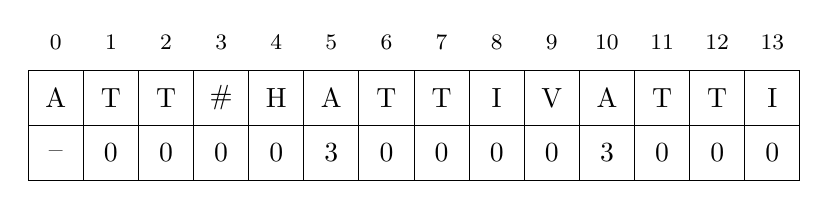
\begin{tikzpicture}[scale=0.7]
\draw (0,0) grid (14,2);

\node at (0.5, 1.5) {A};
\node at (1.5, 1.5) {T};
\node at (2.5, 1.5) {T};
\node at (3.5, 1.5) {\#};
\node at (4.5, 1.5) {H};
\node at (5.5, 1.5) {A};
\node at (6.5, 1.5) {T};
\node at (7.5, 1.5) {T};
\node at (8.5, 1.5) {I};
\node at (9.5, 1.5) {V};
\node at (10.5, 1.5) {A};
\node at (11.5, 1.5) {T};
\node at (12.5, 1.5) {T};
\node at (13.5, 1.5) {I};

\node at (0.5, 0.5) {--};
\node at (1.5, 0.5) {0};
\node at (2.5, 0.5) {0};
\node at (3.5, 0.5) {0};
\node at (4.5, 0.5) {0};
\node at (5.5, 0.5) {3};
\node at (6.5, 0.5) {0};
\node at (7.5, 0.5) {0};
\node at (8.5, 0.5) {0};
\node at (9.5, 0.5) {0};
\node at (10.5, 0.5) {3};
\node at (11.5, 0.5) {0};
\node at (12.5, 0.5) {0};
\node at (13.5, 0.5) {0};

\footnotesize
\node at (0.5, 2.5) {0};
\node at (1.5, 2.5) {1};
\node at (2.5, 2.5) {2};
\node at (3.5, 2.5) {3};
\node at (4.5, 2.5) {4};
\node at (5.5, 2.5) {5};
\node at (6.5, 2.5) {6};
\node at (7.5, 2.5) {7};
\node at (8.5, 2.5) {8};
\node at (9.5, 2.5) {9};
\node at (10.5, 2.5) {10};
\node at (11.5, 2.5) {11};
\node at (12.5, 2.5) {12};
\node at (13.5, 2.5) {13};
\end{tikzpicture}
\end{center}

位置 5 和 10 的值均为 3，这表示模式串 \texttt{ATT} 出现在 \texttt{HATTIVATTI} 的相应位置。

所得算法的时间复杂度为线性，因为只需构造 Z 数组并遍历其中的元素。

\subsubsection{实现}

下面是 Z 算法的简短实现，返回一个表示 Z 数组的向量。

\begin{lstlisting}
vector<int> z(string s) {
    int n = s.size();
    vector<int> z(n);
    int x = 0, y = 0;
    for (int i = 1; i < n; i++) {
        z[i] = max(0,min(z[i-x],y-i+1));
        while (i+z[i] < n && s[z[i]] == s[i+z[i]]) {
            x = i; y = i+z[i]; z[i]++;
        }
    }
    return z;
}
\end{lstlisting}
